\section{Introduction} % (fold) \label{sec:introduction}

A data warehouse is a database specifically used for reporting; thus it is optimized for reducing query response time and not for the insertion, updating or
deletion of records. Data warehouses tend to be much larger than operational databases, often hundreds of gigabytes to terabytes in
size~\cite{chau:db-tech-dss}. Data warehouses are often structured as multidimensional models. These models are often considered more appropriate for Online
Analytical Processing (OLAP) applications than schemas normalized to the third normal form (3NF). Multidimensional models allow the creation of OLAP cubes and
have important benefits for business intelligence in query performance and understandability. In query performance, the number of join operations is greatly
reduced when using a multidimensional cube as opposed to a 3NF model. Furthermore, the query plan can be improved through ``star joins'' which may be performed
faster through indexing or result set size prediction. Finally, multidimensional models are generally easier to understand, allowing the domain specialists and
not the IT professionals to perform the data analysis~\cite{KaserKeithLemire2006}.

Data warehouses are often used as one of the main components of Decision Support Systems~\cite{chau:db-tech-dss}. These systems allow a business to make better
decisions by allowing efficient analyses on historical data accumulated over time. Decision support systems often involve creating OLAP cubes which allow the
efficient analysis of the data acquired from the data warehouse~\cite{pede:md-db-tech}. However, OLAP cubes and data warehouses are also used in other fields
that generate a great number of records. The project presented in this report is geared towards applying data warehousing in the field of literary texts. It is
inspired from the LitOLAP project~\cite{KaserKeithLemire2006} and other related work that combine Natural Language Processing (NLP) and data warehousing
techniques~\cite{inok:OLAP-text-cikm07,text-mining-survey-sigmod07, pere:integratingDW}. The LitOLAP project seeks to apply data warehousing techniques to
literary text processing. It gathers from text the data required to build OLAP cubes that facilitate the analysis of specific aspects of texts that can be
measured. For instance, a cube could be built on the frequencies of co-occurring words, word n-grams or analogies. The OLAP cube generated may help a literary
researcher draw conclusions about an author’s style, or particularities about a book.

My project involves building a data warehouse of places mentioned in books gathered from the Gutenberg Canada website (\url{http://gutenberg.ca/}) and building
a corresponding OLAP cube to facilitate analysis of the data warehouse. For the ETL process, I used: GATE (\url{http://gate.ac.uk/}) to perform Natural
Language Processing (NLP), Nokogiri an XML parser for ruby (\url{http://nokogiri.org/}), and Pentaho’s ETL tool, Kettle (\url{http://pentaho.com/}). As my
RDBMS, I used MySQL. Finally, for my reporting tool and the construction of OLAP cubes I used JasperServer 4.0 (\url{http://jasperforge.org/}) which provides
an installation of Mondrian and JPivot.

% section introduction (end)

\section{Star Schema Design} % (fold)
\label{sec:star_schema}

To build OLAP cubes I used the multidimensional model which is a technique for structuring data so that it is intuitive to business users and delivers fast
query performance. The multidimensional model divides the data between measurements and context. The measurements are captured by the organization's business
processes and are usually numeric. The context is represented by the dimensions which help answer the questions of who, what, when, where, why, and how of a
measurement. Dimensional models may be stored as star schemas or cubes. When stored in a relational database platform, they are called star schemas, and when
stored in an OLAP structure they are called cubes. To illustrate with an example, consider the multidimensional model for a store that sells fish (see
Figure~\ref{fig:figures_FishMDModel}).

\begin{figure}[htbp]
    \centering
        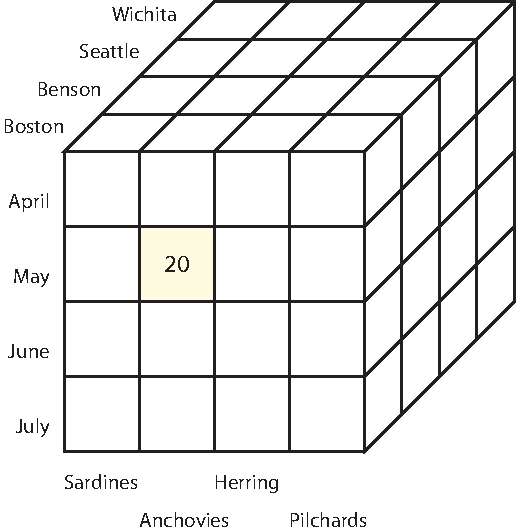
\includegraphics[height=3in]{figures/FishMDModel.pdf}
    \caption{Multidimensional model for a store that sells fish. The measure $20$ Units sold is contextualized by the values specified in each dimension. Thus, we know that $20$ units of Anchovies were sold on May in Boston.}
    \label{fig:figures_FishMDModel}
\end{figure}

Each cell in this model of three dimensions contains a measure. The measure is referenced by specifying a value in each of the three dimensions.
Multidimensional models are often considered more appropriate for OLAP applications than traditional normalized relational models. Because industry also refers
to them as entity-relationship (ER) models, I will refer to them as such. In contrast to multidimensional models, ER models seek to reduce redundancies as much
as possible, and are considered better for transactional processing or Online Transactional Processing (OLTP) applications. The key difference between them is
the degree of normalization. While ER models are completely normalized to third normal form (3NF), the star schema consists of a fact table that is
normalized to 3NF, and dimension tables that are normalized to 2NF. Fact tables are normalized to 3NF because the related context is moved to dimension tables.
The dimension tables connect to the fact table via foreign keys providing the glue of the measurements to their context.

Because the tables for my OLAP cube are stored in a relational database, I am essentially designing a star schema. In my schema, I keep a fact table of places
mentioned in sentences, where the measurement is the number of occurrences of a given place in a sentence. My star schema also consists of two dimensions
tables, namely, place and sentence (see Figure~\ref{fig:figures_MyStarSchema}).

\begin{figure}[bp]
    \centering
        \includegraphics[height=1.8in]{figures/MyStarSchema.pdf}
    \caption{Star schema with sentence and place dimension tables.}
    \label{fig:figures_MyStarSchema}
\end{figure}

\subsection{The Place Dimension} % (fold)
\label{sub:the_place_dimension}

As can be observed from (Figure~\ref{fig:figures_MyStarSchema}), the place dimension table has a hierarchy that goes from finest granularity at city and
coarsest at continent. However, one of the issues of the star schema I propose is that the place mentioned could be at a level different from the lowest level
of the hierarchy. Kimball recommends that every fact in a fact table should be at the grain; the finest granularity in all the hierarchies of its respective
dimensions~\cite{kimball2002dwt}. Because of the nature of the problem, I cannot comply with this advice. A sentence may mention a place that could be a
continent or a country without specifying the country or city in question. Thus, I have some facts that cannot be drilled down to finer details. The issue
may be resolved by creating a dummy value, namely, ``unspecified'' to fill in spots where a member would be missing. While you can still drill down to
unspecified values, these values indicate that a fact is not meant to be interpreted at that level (see Figure~\ref{fig:figures_UnspecifiedValue}).

\begin{figure}[htbp]
    \centering
        \includegraphics[height=1.2in]{figures/UnspecifiedValue.pdf}
    \caption{Place dimension table with ``unspecified'' members for unknown members of the hierarchy}
    \label{fig:figures_UnspecifiedValue}
\end{figure}

Yet another issue I encounter with the place dimension is that there could be ambiguity with cities that could be associated to more than one country. For
instance, London is the name of a city in England and in Canada. In which of these two countries is the mentioned city located? To answer this question more
context from the book would be necessary. This job could potentially be done through further natural language processing. Yet how much context do we need to
figure out to which country does the mentioned city belong? The answer to this question is relative to how much context the book provides and the process used
for determining that context.

Another method to deal with this issue is through allocation. I could assign a fraction of the measurement to two different facts that roll-up to each of the
possible parent members. For example, when given the city London in a sentence, two facts would be created. One would roll up to England, and the other would
roll up to Canada. The fraction of frequency Canada and England would get could be determined through their probabilities. This approach, however, could only
be meaningful for certain queries where the data is summarized at the higher levels of the hierarchy. Querying for which specific books mention London in
Canada, and which mention London in England would not be possible.

% subsection the_place_dimension (end)

\subsection{The Sentence Dimension} % (fold)
\label{sub:the_sentence_dimension}

The sentence dimension table also has a hierarchy that goes from finest granularity at sentence and coarsest at author occupation. For the table of sentences I
maintain a surrogate key to provide better time performance.

Sentences can be rolled up to books and books can be rolled up to authors. However, because two or more authors may write a particular book, a many-to-many
relationship exists between both attributes. Ideally, a hierarchy consists of a single parent member and multiple children members forming a one-to-many
relationship. Because two or more author members are parents of a particular book member this relationship becomes a many-to-many relationship. Such a
relationship between attributes could lead to double counting and other unwanted shortcomings. There are various ways to address this problem, some of which I
address in this report:

\begin{itemize}

\item Repeating attribute: This method involves creating an additional column or attribute for each additional parent member a child member has. For instance,
if I have two authors for a particular book then I would have a field for the first author, and a field for the second. One inherent problem from this approach
is that I do not know how many fields I need to ensure that all authors are accounted for. There is also a lot of space wasted because most books have only one
author.

\item Allocation: This method involves repeating each fact for every author of a given book with an additional Sentence ID. Then each author gets a fraction of
the frequency at which a location is found in a sentence. For instance, suppose a given book has four authors and the city Saint John is mentioned in three
different sentences of the book. Each fact of the table for the three sentences mentioning Saint John would be represented in four different facts, each having
a fourth of the frequency. When adding up the frequencies at which Saint John occurred in this book, I would get a total of three sentences. If the measure is
not divided by the number of authors, this would lead to counting each fact 4 times, resulting in a misleading $12$ times where the city Saint John is
mentioned.

\item Bridge Table: This method consists in removing the many-to-many relationship between the attributes by creating a bridge table and an outtrigger table.
The bridge table assigns a single group ID transforming the relationship between the attributes to a many-to-one. The outtrigger table provides further detail
of the group members. In Figure~\ref{fig:figures_BridgeTable}, I illustrate the star schema after building a bridge table to contain the many-to-many
relationship between books and authors. The attribute ``AuthorGID'' allows the book to be associated to a single attribute value, the bridge table specifies
what author IDs comprise the group and the outrigger table gives us the names of those authors.

\begin{figure}[htbp]
    \centering
        \includegraphics[height=3in]{figures/BridgeTable.pdf}
    \caption{Star schema with bridge table}
    \label{fig:figures_BridgeTable}
\end{figure}

\item Creating a dimension: The last method consists in evading the many-to-many relationship by making the author a dimension. Having author as a dimension
changes the grain of the fact table. Instead of looking only at places mentioned in sentences, we now look at places mentioned in sentences written by a
particular author. The design could allow defining a particular author for a given sentence which could be more appropriate for books like the Bible where
different parts of the book are written by different authors. For the books obtained from the Gutenberg Canada website~\cite{GutenbergCanada-url}, it is
possible to determine the author of each particular sentence. Therefore, all mentions of a particular place are accredited to each of the participating
authors. Special care must be taken when interpreting the results of certain queries. For example, when rolling up sentences to books to find the number of
times a place is mentioned in a particular book, a summarized fact of the place and book will be returned for each author. It is sufficient to look at the
aggregated frequency of one author since both authors are given equal credit for each sentence in the book. Adding the frequencies of both authors would result
in double counting. One disadvantage is that the OLAP cube also becomes quite sparse as most books have only one author.

\end{itemize}

% subsection the_sentence_dimension (end)

% section star_schema (end)

\section{The ETL Process} % (fold)
\label{sec:the_etl_process}

Populating the data warehouse from data sources involves a process of three main phases: extracting the data from each source, transforming it to conform to
the warehouse schema and cleaning it, and loading it into the warehouse. This process is known as ETL (Extract, Transform and Load).

The data extraction step often involves extracting data from various data sources. However, in my project I extracted information from a single data source,
the Gutenberg Canada website. From this website, I extracted the books and their metadata. Before the extraction, I cleaned the HTML file of unnecessary text
and tags that could confuse confuse the regular expressions I would eventually use to extract the book's metadata. Once cleansed, the HTML file was parsed
using Nokogiri, and divided in a series of blocks that contain both a link to the book in text format, and the metadata of the book. In each block, the text
files were downloaded onto disk for later Natural Language Processing (NLP) andthe html in the block is scanned with regular expressions matching the syntax
patterns around information like author, title, occupation, and date.

The transformation process uses a set of rules and scripts to convert the data from an input schema to a destination schema representation. Most of the work in
my ETL process was done on this stage. This stage begins with data cleaning which involves fixing errors and differences in schema conventions. Differences on
such conventions may result on inaccurate query responses and consequently inaccurate mining models. In my project, I had to remove preliminary common
information irrelevant to the content from the books. The transformation process is followed by determining the language of a text as I did not account for
books that were not written in English. I then used GATE, an open-source software for Natural Language Processing (NLP), to annotate the texts with sentence
and place tags. The annotated text is saved as an XML file which is then fed to a script in ruby that builds a de-normalized table using the metadata obtained
during the extraction stage, and the annotations in the XML file. 

Once the de-normalized table is built it is loaded on Pentaho's ETL tool (a.k.a. Kettle) which takes the information and creates and populates the fact and
dimension tables for the schema; thus completing the transformation and loading stages of the ETL Process. The entire transformation process to gather the
sentences and places from the books is illustrated in Figure~\ref{fig:figures_BookETLProcess}.

\begin{figure}[htbp]
    \centering
        \includegraphics[height=3in]{figures/BookETLProcess.pdf}
    \caption{ETL Process for books downoaded from the Gutenberg Canada website.}
    \label{fig:figures_BookETLProcess}
\end{figure}

\subsection{Natural Language Processing} % (fold)
\label{sub:natural_language_processing}

One of the most critical steps in my transformation process was that of doing Natural Language Processing (NLP) for the texts I had downloaded. I did part of
this transformation process with GATE~\cite{gate-url}, and part of it with WhatLanguage~\cite{whatlanguage-url}, a ruby library to detect the language of a
text. Both are free open-source software projects. To begin the process, I used WhatLanguage to determine the language a text is written in. If the text was
written in English I kept it, and if it was not I discarded it. Once I had all texts that were written in English, I used GATE to annotate them. GATE build an
XML file of the English texts where sentences and places are tagged. Sentences are tagged using GATE’s default sentence splitter, and places are tagged using a
Gazetteer. I illustrate the transformation of a text to xml annotated text by GATE in Figure~\ref{fig:figures_AnnotatedXML}.

\begin{figure}[htbp]
    \centering
        \includegraphics[height=2in]{figures/AnnotatedXML.png}
    \caption{Book text transformation process with GATE to XML annotated text.}
    \label{fig:figures_AnnotatedXML}
\end{figure}

% subsection natural_language_processing (end)

\subsection{The Incremental ETL Process} % (fold)
\label{sub:the_incremental_etl_process}

Data warehouses are initially populated with historical data. Then as new data arrives to the data sources, it is updated using an incremental ETL Process. The
process is essentially the same with the exception that it must identify new data. Though I did not plan on implementing this part of the ETL process, I
describe it in this section. In order to perform the incremental ETL Process I would first take the latest html file found in the Gutenberg Canada website and
use the diff command line utility to compare it with the previous html file kept on local disk. Using the output from the diff tool I would determine what
content is new in my file, and generate a file with that new content only. After that, I would run the entire ETL Process previously described with the file
containing the new content in the website.

% subsection the_incremental_etl_process (end)

% section the_etl_process (end)
\section{MDX Queries} % (fold)
\label{sec:mdx_queries}

To generate the OLAP cube from my star schema I use Mondrian--an OLAP server that allows OLAP cube creation from a DBMS such as MySQL. To navigate the cube the
MultiDimensional eXpressions (MDX) query language is used. MDX may look similar to SQL in syntax, but it is quite different. Unlike SQL that allows you to
insert, update and delete, MDX only allows querying information. Rows and columns serve different purposes in SQL and MDX. In SQL rows represent records, and
columns represent attributes of a table. In MDX, rows and columns are both display axises where dimensions can be placed. When a dimension is placed on the
rows, every member of the dimension is listed as a row. In MDX, the cells of the table are not attribute values like in a SQL table but the measurement
obtained when different members of the dimensions of the cube intersect. Consequently, the SELECT and WHERE clauses serve a different purpose as well. SELECT
in SQL is used to determine what attributes to display and WHERE is used to filter the records the user wants to display. The SELECT clause in MDX is used to
define where the dimensions are going to be displayed in columns or rows, and the WHERE clause is used to slice on a particular dimension or define what
measurement to use. In the following sections I cover some concepts and functionality found in MDX and how I apply them to summarize the data in my OLAP Cube.

\subsection{The ``All Members'' Member} % (fold)
\label{sub:the_all_member_}

In MDX, every dimension has a topmost hierarchical member named ``All Members''. The ``All Members'' is the sole member of the topmost level of the hierarchy
and it contains every other level~\cite{Whitehorn:2005:FTM:1098716}. When rolling up to this level all measures associated to the members of the dimension are
aggregated. In the query shown in Listing~\ref{lst:allmembersquery} I put the place dimension on the columns, and the sentence dimension on the rows. Since I
am using the ``All Sentences'' and ``All Places'' members of both dimensions all the occurrences of all places in all sentences are aggregated. The function by
which frequencies are aggregated is count.

\begin{lstlisting}[label=lst:allmembersquery,caption=MDX query using ``All Members'']
SELECT {[Place].[All Places]} ON COLUMNS, 
{[Sentence].[All Sentences]} ON ROWS 
FROM [Places] 
WHERE [Measures].[frequency] 
\end{lstlisting}

However, because the fake value NONE is used, this is misleading as non-occurrences of places in sentences are also accounted for. I can also query
for the occurrences of the place called NONE in all sentences (see Listing~\ref{lst:nonememberquery} ). By subtracting these two resulting measures I can
obtain the total number of occurrences of all places in all sentences.

\begin{lstlisting}[label=lst:nonememberquery,caption=MDX query for all occurrences of NONE]
Select [Place].[NONE] ON COLUMNS,
  {[Sentence].[All Sentences]} ON ROWS
from [Places]
where [Measures].[frequency]
\end{lstlisting}

% subsection the_all_member_ (end)

\subsection{Tuples and Sets} % (fold)
\label{sub:tuples_and_sets}

Specific tuples can also be queries from the cube. A tuple is the intersection of specific members of the dimensions that conform the cube. The members do not
have to be at the finest granularity. In the query illustrated in (listing x), I specify the book \emph{The Black Hunter} from the sentence dimension and the
member ``America'' from the place dimension. Notice that in the sentence dimension I drill down from all sentences to author ``Curwood, James Oliver'', and
from author to the book \emph{The Black Hunter}. Also, the frequency measure is placed on the columns of the cube.

MDX also allows the selection of sets. A set is a collection of 0 or many tuples. In the query in Listing~\ref{lst:setquery}, I select the first $10$ sentences
from the book ``The Black Hunter'' on the columns and ``All Places'' on the rows of the cube. When the NON EMPTY clause is used on rows and columns, empty rows
and columns are eliminated from the selection. If the NON EMPTY clause is omitted from the query, then all possible places are displayed on the rows of the
cube, and all ten sentences are also displayed.

More advanced queries in MDX allow defining a set before use. In the query shown in Listing~\ref{lst:topplacesquery}, the set TopPlaces is defined with the
function TopCount as the top $10$ places occurring in all the sentences of the data warehouse. The function TopCount takes three parameters: a set, a limit,
and a measure. The set is the resulting set after using the \emph{Except} function to remove the place called NONE from ``All Places''. The limit is $10$
because I want the top $10$ places and the measure is the frequency. Members may also be defined before use in a query as shown in
Listing~\ref{lst:validplacesquery}. In this query, after the defining the set ValidPlaces as all places without the place NONE, the member AllValidPlaces is
created as the sum of all the measures referenced by the members of ValidPlaces set. This query responds to the same question as the first two queries
presented in Section~\ref{sub:the_all_member_}, but uses a single query instead of two.

\begin{lstlisting}[label=lst:tuplequery,caption=MDX query for obtaining a single tuple]
SELECT ([Place].[America], 
[Sentence].[All Sentences].[Curwood, James Oliver].[The Black Hunter.]) ON ROWS, 
([Measures].[frequency]) ON COLUMNS 
FROM [Places] 
\end{lstlisting}

\begin{lstlisting}[label=lst:topplacesquery,caption=MDX query to obtain top 10 occurring places]
WITH SET  TopPlaces  AS 'TopCount( Except( {[Place].[All Places].Children}, {[Place].[NONE]}), 10, [Measures].[frequency])'

SELECT NON EMPTY {[Sentence].[All Sentences]} ON COLUMNS,
TopPlaces ON ROWS 
FROM [Places]
WHERE [Measures].[frequency]
\end{lstlisting}

\begin{lstlisting}[label=lst:validplacesquery,caption=MDX query to obtain total number of occurrences of places]
WITH SET ValidPlaces AS 'Except({[Place].[All Places].Children}, {[Place].[NONE]})'
MEMBER [Place].[AllValidPlaces] AS SUM( ValidPlaces , [Measures].[frequency] )

SELECT Hierarchize([Place].[AllValidPlaces]) ON COLUMNS,
  {[Sentence].[All Sentences]} ON ROWS
FROM [Places]
WHERE [Measures].[frequency]
\end{lstlisting}

\begin{lstlisting}[label=lst:setquery,caption=MDX Query for a set]
SELECT NON EMPTY Hierarchize
( {
      [Sentence].[Moodie, Susanna].[Roughing it in the Bush; or, Forest Life in Canada].[0-19].[0], 
      [Sentence].[Moodie, Susanna].[Roughing it in the Bush; or, Forest Life in Canada].[0-19].[1], 
      [Sentence].[Moodie, Susanna].[Roughing it in the Bush; or, Forest Life in Canada].[0-19].[2], 
      [Sentence].[Moodie, Susanna].[Roughing it in the Bush; or, Forest Life in Canada].[0-19].[3], 
      [Sentence].[Moodie, Susanna].[Roughing it in the Bush; or, Forest Life in Canada].[0-19].[4], 
      [Sentence].[Moodie, Susanna].[Roughing it in the Bush; or, Forest Life in Canada].[0-19].[5], 
      [Sentence].[Moodie, Susanna].[Roughing it in the Bush; or, Forest Life in Canada].[0-19].[6], 
      [Sentence].[Moodie, Susanna].[Roughing it in the Bush; or, Forest Life in Canada].[0-19].[7], 
      [Sentence].[Moodie, Susanna].[Roughing it in the Bush; or, Forest Life in Canada].[0-19].[8], 
      [Sentence].[Moodie, Susanna].[Roughing it in the Bush; or, Forest Life in Canada].[0-19].[9]
   } ) ON COLUMNS, 
NON EMPTY Except({[Place].[All Places].Children}, {[Place].[NONE]}) ON ROWS
from [Places]
\end{lstlisting}



% subsection tuples_and_sets (end)




% section mdx_queries (end)